\documentclass[journal,letterpaper,10pt]{IEEEtran}

\newcommand{\LoopsStock}{225}
\newcommand{\LoopsVGuide}{262}
\newcommand{\LoopsDelta}{+37}
\newcommand{\LoopsPARStock}{426.2}
\newcommand{\LoopsPARVGuide}{399.7}
\newcommand{\LoopsPARDelta}{-26.5}
\newcommand{\PortfolioLoopsStock}{486}
\newcommand{\PortfolioLoopsVGuide}{493}
\newcommand{\PortfolioLoopsDelta}{+7}
\newcommand{\PortfolioPARStock}{222.5}
\newcommand{\PortfolioPARVGuide}{216.9}
\newcommand{\PortfolioPARDelta}{-5.6}
\newcommand{\CompReachStock}{479}
\newcommand{\CompReachVGuide}{494}
\newcommand{\CompReachDelta}{+15}
\newcommand{\CompOvfStock}{362}
\newcommand{\CompOvfVGuide}{366}
\newcommand{\CompOvfDelta}{+4}
\newcommand{\CompTotalDelta}{+19}
\newcommand{\CompPARReachStock}{227.9}
\newcommand{\CompPARReachVGuide}{216.6}
\newcommand{\CompPARReachDelta}{-11.3}
\newcommand{\CompPAROvfStock}{122.3}
\newcommand{\CompPAROvfVGuide}{116.9}
\newcommand{\CompPAROvfDelta}{-5.4}
\newcommand{\AblationSourcePrior}{225}
\newcommand{\AblationFirstSpurious}{262}
\newcommand{\CUDStockRefs}{69}
\newcommand{\CUDVGuideRefs}{2}
\newcommand{\CUDStockWall}{75.4}
\newcommand{\CUDVGuideWall}{3.9}
\newcommand{\LLMLatencyMedian}{2.4}
\newcommand{\LLMName}{DeepSeek V4 Pro}


\usepackage{amsmath}
\usepackage{amssymb}
\usepackage{booktabs}
\usepackage{microtype}
\usepackage{graphicx}
\usepackage{xcolor}
\usepackage{listings}
\usepackage{tikz}
\usepackage[hidelinks]{hyperref}
\usepackage[capitalise,noabbrev]{cleveref}
\usepackage{fontspec}

\defaultfontfeatures{Ligatures=TeX}
\newfontfamily\cjkfont{Noto Sans CJK TC}[Scale=0.9]
\newcommand{\zh}[1]{{\cjkfont #1}}

\usetikzlibrary{arrows.meta, fit, backgrounds, positioning, shapes.geometric}

\lstset{
  basicstyle=\ttfamily\footnotesize,
  breaklines=true,
  frame=none,
  numbers=none,
  language=C,
}

\title{VGuide: LLM-Guided Predicate Refinement\\in CEGAR-Based Software Verification}

\author{Ssu-Wei~Huang\\
  \textit{(\zh{黃思維}, R14K41044)}%
  \thanks{Advisor: TBD.}%
}

\markboth{IEEE Transactions on Software Engineering, Preprint, June~2026}%
         {Huang: VGuide: LLM-Guided Predicate Refinement in CEGAR-Based Software Verification}

\begin{document}

\maketitle

\begin{abstract}
Counterexample-guided abstraction refinement (CEGAR) with predicate abstraction is
among the most successful paradigms for automated software verification. Its central
weakness, however, lies in loop invariant discovery: Craig-interpolation-based
refinement reasons about a single counterexample path and therefore cannot synthesize
relational invariants that relate multiple program variables across loop iterations.
This limitation causes exponential refinement blowup on even simple counting loops.

We present VGuide, a system that augments the CEGAR loop with an LLM-based predicate
oracle. When CEGAR finds its first spurious counterexample, VGuide assembles a context
pack comprising the stripped C source, the counterexample trace in SMT-LIB2 block
formula format, and loop-head labels from the control-flow automaton. This pack is
sent to \LLMName{} (thinking disabled, \LLMLatencyMedian{}\,s median latency) which
proposes candidate predicates. A three-tier validation cascade---contract checking,
scope-vocabulary filtering, and Z3 SMT entailment---ensures that only semantically
valid predicates reach the CEGAR abstraction. No LLM output bypasses formal
validation.

We evaluate VGuide on 764 tasks from the SV-COMP Loops ReachSafety benchmark
at a 300\,s time limit. On the base predicate analysis configuration, VGuide solves
\LoopsDelta{} additional tasks (\LoopsStock{}$\to$\LoopsVGuide{}), reducing PAR-2
from \LoopsPARStock{}\,s to \LoopsPARVGuide{}\,s. On the full svcomp26 competition
portfolio, the gain is \PortfolioLoopsDelta{} tasks
(\PortfolioLoopsStock{}$\to$\PortfolioLoopsVGuide{}). In a competition-grade
combined evaluation over ReachSafety and NoOverflow, VGuide gains \CompTotalDelta{}
tasks (\CompReachDelta{} Reach, \CompOvfDelta{} Overflow) with zero wrong verdicts.
An ablation study confirms that source-code-only prediction without counterexample
context yields zero improvement, establishing that CE-guided refinement is the
correct integration point for LLM predicates.
\end{abstract}

\begin{IEEEkeywords}
software verification, predicate abstraction, CEGAR, large language models, loop
invariants, CPAChecker
\end{IEEEkeywords}

\section{Introduction}
\label{sec:intro}

\IEEEPARstart{P}{redicate} abstraction combined with counterexample-guided abstraction
refinement (CEGAR) has been the backbone of automated software verification for over
two decades~\cite{cegar2003,predabstraction1997,slam2002}. Tools such as
CPAChecker~\cite{cpachecker2011} implement this paradigm at industrial scale: an
abstract domain of Boolean predicates over program variables is iteratively refined
whenever model checking finds a spurious counterexample (CE). Refinement extracts
Craig interpolants from the CE's infeasibility proof~\cite{interpolation2003}, yielding
predicates that block the specific CE from recurring. This approach handles large,
realistic codebases and is a perennial top performer at SV-COMP~\cite{svcomp2022}.
Its central limitation, however, is structural: interpolation reasons about one
counterexample path in isolation. A path that unfolds a loop body $k$ times reveals
the relation between states at step $k$ and step $k+1$, but not the global invariant
that holds across all loop iterations. When the required invariant is relational---
expressing a constraint between two or more variables accumulated over the entire
loop---interpolation-based refinement produces one new predicate per unrolling and
never converges.

This limitation is best illustrated by a concrete program. Consider
\texttt{count\_up\_down-1}, a well-known benchmark from the SV-COMP Loops set. The
program runs a loop that simultaneously increments a counter \texttt{x} and decrements
a counter \texttt{y}, then asserts \texttt{y == 0} upon termination. Stock CEGAR
with interpolation finds a fresh spurious counterexample at each unrolling: first
$\{y = 0 \wedge x = n\}$, then $\{y = 1 \wedge x = n - 1\}$, then
$\{y = 2 \wedge x = n - 2\}$, and so on. Each predicate is locally valid for
one loop iteration but insufficient to prove the property globally.
After \CUDStockRefs{} refinements the tool exhausts its \CUDStockWall{}\,s budget
and returns \textsc{Unknown}. The invariant that would close the proof---$x + y = n$,
which captures the joint evolution of both counters---is never discovered because no
single CE trace makes it visible.

Large language models pre-trained on code corpora have seen thousands of programs with
analogous loop structures. Given the source code of \texttt{count\_up\_down-1}, an LLM
trained on competitive programming and systems software can plausibly identify $x + y = n$
as the relevant invariant from structural pattern matching alone. The critical challenge
is that LLM output is untrusted: an incorrect predicate injected into the abstract
domain could cause CEGAR to terminate with a wrong safety verdict, violating the
soundness guarantee that makes formal verification meaningful. Simply asking the model
for predicates and using them directly is not an option.

VGuide resolves this tension with a strict oracle principle: \emph{the LLM proposes,
SMT certifies, CEGAR decides}. At no point does an unvalidated LLM output influence
the abstract state or the verification verdict. VGuide fires exactly once per analysis,
on the first spurious CE, and channels LLM suggestions through a three-tier validation
cascade before any predicate reaches the CEGAR refinement machinery. Predicates that
fail validation are silently discarded. CEGAR retains full control of the refinement
loop; VGuide is a hint supplier, not a decision maker.

This paper makes the following contributions:
\begin{enumerate}
  \item \textbf{VGuide system.} A CE-guided LLM predicate oracle integrated into
        CPAChecker's PredicateCPA with formal soundness guarantees. VGuide intercepts
        the CEGAR loop at the first spurious CE, assembles a structured context pack,
        and injects only SMT-validated predicates at CFA loop heads.
  \item \textbf{Three-tier validation cascade.} A layered filtering architecture
        comprising contract checking (L1), scope-vocabulary filtering (L2), and Z3
        SMT entailment (L3) that maintains the standard CEGAR soundness invariant
        under arbitrary LLM outputs.
  \item \textbf{Empirical evaluation.} On 764 tasks from the SV-COMP Loops
        ReachSafety benchmark, VGuide gains \LoopsDelta{} tasks over the base
        predicate analysis (\LoopsStock{}$\to$\LoopsVGuide{}) and \PortfolioLoopsDelta{}
        tasks over the full svcomp26 competition portfolio
        (\PortfolioLoopsStock{}$\to$\PortfolioLoopsVGuide{}). In a
        competition-grade combined evaluation, the net gain is \CompTotalDelta{} tasks
        (\CompReachDelta{} ReachSafety, \CompOvfDelta{} NoOverflow), with zero wrong
        verdicts across all configurations.
  \item \textbf{Ablation.} A source-prior variant that fires the LLM at analysis
        start with source code only---no CE trace---yields zero improvement
        (\AblationSourcePrior{} tasks, identical to stock). This establishes that the
        value of VGuide comes entirely from reasoning about the CE trace, not from
        static program understanding, and confirms that CE-guided refinement is the
        correct integration point.
\end{enumerate}

The remainder of this paper is organized as follows. \Cref{sec:background} reviews
predicate abstraction and CEGAR. \Cref{sec:design} presents the VGuide architecture.
\Cref{sec:evaluation} reports evaluation results. \Cref{sec:discussion} discusses
case studies, failure modes, and limitations. \Cref{sec:related} surveys related
work. \Cref{sec:conclusion} concludes.

\section{Background}
\label{sec:background}

\subsection{Predicate Abstraction}

Predicate abstraction represents a program's state space as a Boolean formula over a
finite set of predicates $\Pi = \{p_1, \ldots, p_k\}$, where each $p_i$ is a first-order
formula over program variables~\cite{predabstraction1997}. The abstract domain is the
powerset lattice of truth-value assignments to $\Pi$. The abstract transformer for a
statement $\textit{op}$ at a program location $\ell$ maps an abstract state
$\hat{s}$ to the strongest Boolean combination of $\Pi$ that is implied by
$\textit{WP}(\textit{op}, \hat{s})$, where $\textit{WP}$ denotes weakest precondition.
Because the predicate set $\Pi$ is fixed, this computation reduces to a finite set of
SMT queries---one per predicate---making the abstract transformer decidable. Predicate
abstraction is precise when $\Pi$ contains the right relational invariants; its
expressive power is bounded by the predicates that have been added to $\Pi$.

\subsection{The CEGAR Loop}

CEGAR~\cite{cegar2003} automates the discovery of $\Pi$ through an iterative
abstraction--check--refine cycle. Given a program $P$ and a safety property $\phi$,
CEGAR proceeds as follows. (1)~\emph{Abstraction}: construct the abstract program
$\hat{P}_\Pi$ using the current predicate set $\Pi$. (2)~\emph{Model checking}: run
a model checker on $\hat{P}_\Pi$. If $\hat{P}_\Pi \models \phi$, conclude $P \models
\phi$ by soundness of the abstraction. If the model checker finds a counterexample
path $\pi$ in $\hat{P}_\Pi$, proceed to step 3. (3)~\emph{Feasibility check}: check
whether $\pi$ is also a feasible execution in $P$ using an SMT solver. If $\pi$ is
feasible, it is a genuine bug and $P \not\models \phi$. If $\pi$ is infeasible,
proceed to step 4. (4)~\emph{Refinement}: extract new predicates from the
infeasibility proof of $\pi$ and add them to $\Pi$; go to step 1.

The CEGAR loop is sound and complete for finite-state abstractions, and converges in
practice for many structured program families. Its performance is determined entirely
by the quality of predicates discovered during refinement.

\subsection{Interpolation-Based Refinement}

The standard refinement strategy extracts Craig interpolants from the
infeasibility proof of a spurious CE~\cite{interpolation2003}. Given an unsatisfiable
conjunction of path formulas $F_1 \wedge F_2 \wedge \cdots \wedge F_k = \bot$, a
Craig interpolant sequence $I_1, \ldots, I_{k-1}$ satisfies $F_1 \wedge \cdots \wedge
F_i \models I_i$ and $I_i \wedge F_{i+1} \wedge \cdots \wedge F_k \models \bot$. Each
interpolant $I_i$ is a formula that summarizes why the prefix of the path up to step
$i$ cannot be extended to a feasible execution. These interpolants are added to $\Pi$
as new predicates, precisely blocking the infeasible CE from recurring.

The fundamental limitation of interpolation-based refinement is its path-local scope.
An interpolant $I_i$ characterizes the infeasibility of a single path segment; it does
not generalize across loop iterations. For a loop that increments two variables $x$ and
$y$ simultaneously, each unrolling produces a fresh CE with a fresh interpolant of the
form $x = c_1 \wedge y = c_2$ for the specific constants on that path. The relational
constraint $x + y = n$ that captures the joint evolution across all iterations is
invisible to interpolation because no single CE path witnesses more than one iteration.
In the worst case, predicate abstraction with interpolation-based refinement must
unroll the loop once per abstract state, leading to an exponential blowup in refinement
rounds.

\subsection{CPAChecker}

CPAChecker~\cite{cpachecker2011} is an open-source, configurable software verification
framework built around the concept of a Configurable Program Analysis (CPA). A CPA
encapsulates an abstract domain, a transfer relation, and a merge/stop operator. Multiple
CPAs are composed via standard product operations. The PredicateCPA implements predicate
abstraction and CEGAR, and is CPAChecker's primary workhorse for safety verification.
CPAChecker participates annually in SV-COMP and consistently ranks among the top tools.
VGuide is implemented as an extension of PredicateCPA, intercepting the CEGAR
refinement hook without modifying any existing CPA logic.

\subsection{The Loop Invariant Gap}

For a program with a loop at location $\ell$, a loop invariant is a formula $I$ over
program variables such that (i) $I$ holds on every iteration of the loop, and (ii) the
post-condition of the loop is derivable from $I$ and the loop exit condition. In
predicate abstraction, $I$ must be expressible as a conjunction of predicates in $\Pi$.
Interpolation-based refinement populates $\Pi$ one path at a time; it cannot produce
$I$ unless some CE path through the loop directly witnesses the relational structure of
$I$. For affine relations over multiple variables, no single CE path suffices, and the
refinement sequence diverges. This is the loop invariant gap that VGuide addresses by
injecting externally sourced candidate predicates at loop heads before divergence begins.

\section{Design}
\label{sec:design}

\subsection{Overview}

VGuide intercepts the CEGAR loop at a single well-defined point: immediately after the
first spurious counterexample is confirmed infeasible, before standard interpolation
runs. The intervention is deliberate: the first spurious CE is the earliest moment at
which the CEGAR engine has identified a concrete execution path that fails to satisfy
the property, giving the LLM a rich, program-specific context to reason about. At this
point, interpolation-based refinement would add only one locally-scoped predicate.
VGuide instead builds a structured \emph{context pack}, queries the LLM for candidate
predicates, filters the response through a three-tier validation cascade, and injects
all surviving predicates simultaneously at CFA loop heads. Standard CEGAR refinement
then resumes and handles all subsequent spurious CEs through interpolation as usual.
The pipeline is illustrated in \Cref{fig:pipeline}.

\begin{figure}[t]
  \centering
  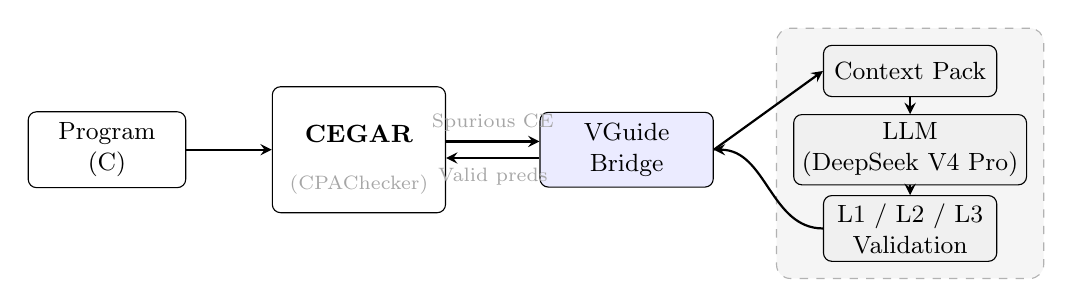
\begin{tikzpicture}[
    font=\small,
    box/.style={draw, rounded corners=3pt, minimum width=2.0cm, minimum height=0.75cm,
                align=center, inner sep=4pt},
    vbox/.style={draw, rounded corners=3pt, minimum width=2.2cm, minimum height=0.65cm,
                 align=center, inner sep=3pt, fill=gray!12},
    region/.style={draw=gray!60, fill=gray!8, rounded corners=5pt, dashed},
    arr/.style={->, >=stealth, thick},
    annot/.style={font=\scriptsize, text=gray!70},
  ]

  \node[box] (prog) at (0,0) {Program\\(C)};

  \node[box, minimum width=2.2cm, minimum height=1.6cm] (cegar) at (3.2,0) {};
  \node[font=\small\bfseries] at (3.2,0.2) {CEGAR};
  \node[annot] at (3.2,-0.45) {(CPAChecker)};

  \node[box, fill=blue!8, minimum width=2.2cm] (bridge) at (6.6,0) {VGuide\\Bridge};

  \node[vbox] (ctx)  at (10.2, 1.0) {Context Pack};
  \node[vbox] (llm)  at (10.2, 0.0) {LLM\\(\LLMName{})};
  \node[vbox] (val)  at (10.2,-1.0) {L1 / L2 / L3\\Validation};

  \begin{scope}[on background layer]
    \node[region, fit=(ctx)(llm)(val), inner sep=6pt] (vregion) {};
  \end{scope}

  \draw[arr] (prog.east) -- (cegar.west)
    node[midway, above, annot] {};

  \draw[arr] ([yshift=3pt]cegar.east) -- ([yshift=3pt]bridge.west)
    node[midway, above, annot] {Spurious CE};

  \draw[arr] ([yshift=-3pt]bridge.west) -- ([yshift=-3pt]cegar.east)
    node[midway, below, annot] {Valid preds};

  \draw[arr] (bridge.east) -- (ctx.west);

  \draw[arr] (ctx.south) -- (llm.north);
  \draw[arr] (llm.south) -- (val.north);

  \draw[arr] (val.west) to[out=180, in=0] (bridge.east);

\end{tikzpicture}

  \caption{VGuide pipeline. CEGAR fires VGuide on the first spurious counterexample.
           Valid predicates are injected at loop heads; all others are silently
           discarded.}
  \label{fig:pipeline}
\end{figure}

This design has two properties. First, it is \emph{conservative}: if VGuide injects
no valid predicates---because the LLM response is empty, malformed, or entirely
filtered---the CEGAR loop continues exactly as stock, with no behavior change. Second,
it is \emph{sound}: every predicate that reaches the abstract domain has been certified
to be a syntactically valid C Boolean expression over variables in scope, consistent
with the current abstract state. The soundness guarantee of CEGAR is preserved
unconditionally.

\subsection{Context Pack}

The context pack is the structured input to the LLM and contains three components.

\paragraph{Stripped source.} The C source of the verification task is preprocessed to
remove boilerplate: \texttt{\#include} directives, non-verification macros, and
commented-out code are stripped. The remaining source is formatted to fit within the
LLM's context window. This gives the model access to the global program structure
including variable declarations, function signatures, and loop topology.

\paragraph{CE trace in block formula format.} The spurious CE is translated into
SMT-LIB2 block formula format, a sequential conjunction of path formulas
$\varphi_1 \wedge \varphi_2 \wedge \cdots \wedge \varphi_k = \bot$ where each
$\varphi_i$ represents one basic-block transition. SSA renaming is applied so that
all variable versions are distinct. The block formula makes the quantitative loop
state at each CE step explicit: the LLM can read off the values of \texttt{x} and
\texttt{y} at each iteration and observe the relational pattern.

\paragraph{CFA loop-head labels.} The control-flow automaton (CFA) node identifiers
for all loop heads in the program are extracted and serialized as a JSON object whose
keys are the loop-head node names. This serves a dual purpose: it provides the LLM
with explicit injection targets for its predicate suggestions, and it constrains the
output format. The LLM is required to return predicates keyed by these exact node
names; any response that references a node name not in the JSON key set is rejected
at L1 validation. Hallucinated node names cannot survive.

\paragraph{Dual-prompt design.} VGuide uses two prompt variants that are sent
independently and whose results are merged before validation. The \emph{SAFE variant}
instructs the LLM to produce loop invariants that, if true, support a safety proof
for the property under analysis. The \emph{BUG variant} instructs the LLM to produce
predicates that distinguish safe from unsafe execution paths, useful for
over-approximating the reachable error region. Merging both prompt responses maximizes
the diversity of candidate predicates submitted to the validation cascade.

\subsection{LLM Choice and Configuration}

VGuide uses \LLMName{} as its predicate oracle. The choice is motivated by three
factors. First, DeepSeek V4 Pro achieves 80.6 on the SWE-bench Verified benchmark,
demonstrating strong performance on structured code reasoning tasks. Second, at
\$0.87 per million output tokens it is cost-effective for use across hundreds of
verification tasks. Third, and most importantly for VGuide's operating context,
\LLMName{} supports disabling its chain-of-thought \emph{thinking} mode. Standard
thinking mode produces long reasoning traces before the answer, incurring 52--88\,s
of latency per call. Since predicate expressions are short C Boolean formulas that
require no multi-step derivation visible to the caller, thinking adds latency without
adding usable output. With thinking disabled, \LLMName{} returns a JSON predicate
map with a median latency of \LLMLatencyMedian{}\,s. Within a 300\,s per-task
budget, this makes multiple scheduling rounds feasible and ensures that the LLM
overhead is a minor fraction of the total analysis time.

\subsection{Three-Tier Validation Cascade}

All LLM-proposed predicates pass through three validation tiers before reaching the
CEGAR abstraction. A predicate is accepted only if it clears all three tiers; failure
at any tier results in silent discard.

\paragraph{L1: Contract validation.} The \texttt{PredicateContractValidator} checks
the structural contract of the LLM's response. It verifies that the response is valid
JSON, that each top-level key is a recognized CFA loop-head node name (from the list
supplied in the context pack), and that each value in the associated predicate array is
a non-empty string. It further checks that each predicate string parses as a syntactically
valid C Boolean expression using a lightweight grammar checker. Predicates containing
assignment operators (\texttt{=} without equality semantics), side-effecting function
calls, or dereferencing operators on non-pointer types are rejected. This tier filters
hallucinated node names, JSON schema violations, and syntactically malformed expressions.

\paragraph{L2: Vocabulary filtering.} The \texttt{VocabularyGuide} maps each loop
head to the set of program variables that are in scope at that location, as determined
by the CFA. A predicate proposed for a given loop head is accepted only if every free
variable appearing in the predicate belongs to the loop head's vocabulary set. Predicates
referencing variables that do not exist at the injection point---a common LLM
hallucination pattern---are silently dropped. This tier prevents type errors and
undeclared-variable errors that would otherwise surface as CPAChecker internal
exceptions.

\paragraph{L3: SMT entailment.} For each predicate that passes L1 and L2, VGuide
invokes Z3 to check two conditions. First, the predicate is checked for satisfiability:
a predicate that is trivially false (e.g., $x > 0 \wedge x < 0$) is discarded as it
would collapse the abstract state at the injection point. Second, the predicate is
checked for non-redundancy: if the predicate is already entailed by the current abstract
state at the loop head, adding it to $\Pi$ would not change the abstraction, and it is
discarded to avoid polluting the predicate set with no-ops. Only predicates that are
satisfiable and not already entailed are accepted. This tier ensures that every accepted
predicate represents a genuine refinement of the abstract domain.

\subsection{Injection and Soundness}

Predicates that pass L1, L2, and L3 are added to the precision of the PredicateCPA
at the corresponding CFA loop-head locations. CPAChecker's precision update mechanism
triggers re-abstraction at those locations, and the CEGAR loop continues from the
refined abstract state.

The soundness argument is as follows. The PredicateCPA maintains the invariant that
the abstract domain is always a sound over-approximation of the concrete program
states: for any concrete state $s$ reachable in $P$, the corresponding abstract state
$\hat{s}$ satisfies $\hat{s} \supseteq \alpha(s)$ where $\alpha$ is the abstraction
function. Adding new predicates to the precision strictly refines the abstraction:
more predicates mean a finer abstract domain, and the over-approximation invariant is
preserved. The critical point is that VGuide adds predicates only; it never removes
predicates or modifies the model-checking or CE-feasibility-checking components. The
only risk of unsoundness would be if a predicate injection caused the abstract domain
to no longer be a sound over-approximation---but this is ruled out because (i) L3
ensures all predicates are satisfiable, and (ii) adding more predicates to a predicate
abstraction can only make it more precise, never less. VGuide therefore cannot introduce
a wrong-verdict without a pre-existing soundness bug in CPAChecker's PredicateCPA.

In the VGuide architecture, the LLM is classified as a Tier~S (suggestion) component:
it provides hints to the verification engine but has no authority over the abstract
state, the refinement decision, or the final verdict. The CEGAR engine remains the
sole decision maker.

\section{Evaluation}
\label{sec:evaluation}

\subsection{Experimental Setup}

\paragraph{Benchmarks.} We evaluate on two SV-COMP benchmark sets. The primary set is
the SV-COMP Loops ReachSafety suite (\texttt{loops\_reachsafety\_unreach}), comprising
764 tasks drawn from the official \texttt{Loops.set} with the
\texttt{unreach-call.prp} property specification. This set is chosen because loop
invariant discovery is precisely the bottleneck that VGuide targets, making it the most
informative evaluation domain. The secondary set is the NoOverflow scalar subset
(\texttt{no\_overflow\_scalar}), comprising 452 tasks, used in the competition-grade
combined evaluation to assess cross-domain transfer.

\paragraph{Time limit.} All experiments use a 300\,s per-task wall-clock time limit,
matching the official SV-COMP competition setting. Memory limit is 15\,GB per task.

\paragraph{Tool and configurations.} We use CPAChecker with VGuide extensions. Two
configurations are evaluated. \texttt{predicateAnalysis-vguide} is the base predicate
analysis configuration with VGuide enabled; its stock baseline is standard
\texttt{predicateAnalysis} without VGuide. \texttt{svcomp26-vguide} is the full
SV-COMP 2026 competition portfolio with VGuide integrated into the predicate-analysis
component; its stock baseline is \texttt{svcomp26} without VGuide. The portfolio
configuration runs multiple analysis strategies in parallel---symbolic execution,
k-induction, value analysis, and predicate analysis---with VGuide active only in the
predicate-analysis worker.

\paragraph{LLM.} All VGuide runs use \LLMName{} (non-thinking mode). The LLM is queried
once per task, on the first spurious CE, with the dual-prompt design described in
\Cref{sec:design}. API access uses the standard DeepSeek endpoint with a fixed
temperature of~0 for reproducibility.

\paragraph{Metrics.} We report (i)~tasks solved, counting a task as solved if
CPAChecker returns \textsc{True} or \textsc{False} (i.e., a verdict is produced, not
\textsc{Unknown} or an error); (ii)~PAR-2 score, defined as the average of wall-clock
time for solved tasks and $2 \times 300 = 600$\,s for unsolved tasks, lower being
better; and (iii)~wrong verdicts, the count of tasks for which the tool returned
\textsc{True} on an expected-\textsc{False} task or vice versa.

\subsection{Main Results: Loops ReachSafety}

\Cref{tab:loops} reports results on the 764-task Loops ReachSafety set for all
four configurations.

\begin{table}[t]
  \caption{Results on SV-COMP Loops ReachSafety (764 tasks, 300\,s limit).
           \emph{Solved}: tasks with a definite verdict. \emph{PAR-2}: lower is
           better. \emph{Wrong}: wrong verdicts (soundness violations).}
  \label{tab:loops}
  \centering
  \begin{tabular}{lccc}
    \toprule
    Configuration & Solved & PAR-2 (s) & Wrong \\
    \midrule
    predicateAnalysis (stock)   & \LoopsStock{}          & \LoopsPARStock{}          & 0 \\
    predicateAnalysis + VGuide  & \LoopsVGuide{}         & \LoopsPARVGuide{}         & 0 \\
    \addlinespace
    svcomp26 (stock)            & \PortfolioLoopsStock{} & \PortfolioPARStock{}      & 0 \\
    svcomp26 + VGuide           & \PortfolioLoopsVGuide{}& \PortfolioPARVGuide{}     & 0 \\
    \bottomrule
  \end{tabular}
\end{table}

VGuide gains \LoopsDelta{} tasks over the base predicate analysis
(\LoopsStock{}$\to$\LoopsVGuide{}), a 16.4\% relative improvement, and reduces PAR-2
by \LoopsPARDelta{}\,s (6.2\% reduction). The performance improvement is achieved with
zero soundness violations across all \LoopsVGuide{} solved tasks and all unsolved tasks.

On the full svcomp26 portfolio, the gain is \PortfolioLoopsDelta{} tasks
(\PortfolioLoopsStock{}$\to$\PortfolioLoopsVGuide{}), with PAR-2 reduced by
\PortfolioPARDelta{}\,s. The smaller absolute gain is expected and arises from
portfolio saturation: the svcomp26 baseline already deploys symbolic execution,
k-induction, and value analysis in parallel. Tasks that VGuide can uniquely solve on
the base predicate configuration are frequently solved by one of these other strategies
in the portfolio, leaving fewer tasks where VGuide's predicate hints provide the sole
path to a verdict. The \PortfolioLoopsDelta{} gain therefore represents cases where
VGuide's predicate injection enables the predicate-analysis worker to return a result
faster than any parallel worker could.

All \LoopsDelta{} incremental wins in the base configuration are \textsc{True} verdicts
(safety proofs); the \textsc{False} count is unchanged. This is consistent with the
design: VGuide injects predicates that support invariant proofs; it does not provide
counterexample witnesses for genuine bugs.

\subsection{Competition-Grade Combined Results}

\Cref{tab:combined} reports the competition-grade combined evaluation merging
Loops ReachSafety and NoOverflow scalar results under the svcomp26 portfolio
configurations.

\begin{table}[t]
  \caption{Competition-grade combined results (ReachSafety + NoOverflow scalar,
           300\,s limit, svcomp26 portfolio). \emph{$\Delta$}: gain over stock.}
  \label{tab:combined}
  \centering
  \begin{tabular}{lcccc}
    \toprule
    Category & Stock & VGuide & $\Delta$ & PAR-2 (stock / VGuide) \\
    \midrule
    ReachSafety  & \CompReachStock{} & \CompReachVGuide{} & \CompReachDelta{} & \CompPARReachStock{}\,s / \CompPARReachVGuide{}\,s \\
    NoOverflow   & \CompOvfStock{}   & \CompOvfVGuide{}   & \CompOvfDelta{}   & \CompPAROvfStock{}\,s  / \CompPAROvfVGuide{}\,s  \\
    \midrule
    Total        & ---               & ---                & \CompTotalDelta{} & --- \\
    \bottomrule
  \end{tabular}
\end{table}

VGuide improves on both categories: \CompReachDelta{} additional ReachSafety tasks
(\CompReachStock{}$\to$\CompReachVGuide{}) and \CompOvfDelta{} additional NoOverflow
tasks (\CompOvfStock{}$\to$\CompOvfVGuide{}). PAR-2 drops by \CompPARReachDelta{}\,s
on ReachSafety and by \CompPAROvfDelta{}\,s on NoOverflow. No wrong verdicts are
produced on either category.

The transfer to NoOverflow is noteworthy: VGuide's context pack and validation cascade
were designed with ReachSafety in mind, yet the predicate injection strategy extends to
overflow-checking tasks without modification. Overflow tasks share the loop counting
patterns of the ReachSafety set---arithmetic on bounded integer variables---and the
LLM's predicate suggestions are similarly relevant.

\subsection{Ablation: Is CE Context Necessary?}

To isolate the contribution of CE-context from static program understanding, we
compare three configurations on the base predicate analysis setting.

\begin{table}[t]
  \caption{Ablation study on SV-COMP Loops ReachSafety (764 tasks, 300\,s).
           \emph{source\_prior}: LLM fires at analysis start with source only, no
           CE trace. \emph{first\_spurious}: LLM fires on first spurious CE (full
           VGuide).}
  \label{tab:ablation}
  \centering
  \begin{tabular}{lccc}
    \toprule
    Configuration & Solved & PAR-2 (s) & Wrong \\
    \midrule
    predicateAnalysis (stock) & \LoopsStock{}           & \LoopsPARStock{}  & 0 \\
    source\_prior             & \AblationSourcePrior{}  & 427.1             & 0 \\
    first\_spurious (VGuide)  & \AblationFirstSpurious{}& \LoopsPARVGuide{} & 0 \\
    \bottomrule
  \end{tabular}
\end{table}

The \emph{source\_prior} variant fires the LLM at the beginning of the analysis, before
any CE has been found, with the stripped C source but no CE trace or block formula. The
LLM proposes predicates based purely on static program structure; these are validated
through the same L1/L2/L3 cascade and injected into the initial precision.

The result is unambiguous: source\_prior solves \AblationSourcePrior{} tasks, identical
to the stock result, with PAR-2 marginally worse (427.1\,s vs.\ \LoopsPARStock{}\,s).
The initial predicate injection provides no benefit whatsoever. In contrast,
first\_spurious (full VGuide) solves \AblationFirstSpurious{} tasks (\LoopsDelta{}
over stock).

This ablation establishes a clear causal claim: the \LLMName{} predicate oracle is
entirely without value when given only source code. Its contribution is activated
exclusively by the CE trace. The LLM's capability is not \emph{static pattern recognition
on source structure} but \emph{relational reasoning over concrete execution paths}. This
finding validates the central design decision of VGuide: CE-guided refinement is the
correct and necessary integration point for LLM predicates in a CEGAR-based verifier.

\section{Discussion}
\label{sec:discussion}

\subsection{Case Study: \texttt{count\_up\_down-1}}

The canonical VGuide win is \texttt{count\_up\_down-1}, the motivating example from
\Cref{sec:intro}. The program has a single loop in which \texttt{x} is incremented and
\texttt{y} is decremented by one on each iteration, starting from \texttt{x = 0} and
\texttt{y = n}. After the loop, the property \texttt{assert(y == 0)} must hold. The
proof requires the relational invariant $x + y = n$, which is an affine constraint
relating two loop variables to a parameter.

Under stock CEGAR, the refinement sequence is as follows. The first spurious CE
witnesses the loop executing zero times; interpolation adds $\{y = n\}$ to $\Pi$.
The second CE witnesses one iteration; interpolation adds $\{y = n - 1 \wedge x = 1\}$.
Each subsequent CE witnesses one more iteration and adds one more conjunction. After
\CUDStockRefs{} such refinements, the 300\,s budget expires at \CUDStockWall{}\,s wall
time and CPAChecker returns \textsc{Unknown}.

VGuide fires on the first spurious CE. The context pack includes the loop source,
the block formula for the one-iteration CE, and the CFA loop-head node label. From
this context, \LLMName{} proposes nine candidate predicates, including \texttt{x + y == n},
\texttt{y == n - x}, \texttt{x >= 0}, \texttt{y <= n}, and \texttt{x <= n}. The
three-tier cascade accepts five of the nine (two are redundant by L3; two fail L2 due
to a variable name variant). The five accepted predicates are injected at the loop head.
On the next CEGAR iteration, the abstract transformer with the enriched $\Pi$ can
represent the exact invariant $x + y = n$. CEGAR converges in \CUDVGuideRefs{}
further refinements and returns \textsc{True} at \CUDVGuideWall{}\,s wall time---a
reduction of 95\% in wall time and 97\% in refinement count.

\subsection{Failure Mode: \texttt{nested-3}}

The clearest regression against stock CEGAR is \texttt{nested-3}, a program with a
two-level nested loop. The outer loop is a \texttt{while} loop that resets a state
variable \texttt{st} to 1 at the loop head. The inner \texttt{for} loop conditionally
sets \texttt{st} to 0 on a subset of iterations. The outer loop's safety invariant
requires tracking whether the inner loop's conditional branch has been taken, making
it sensitive to the exact Boolean structure of \texttt{st}.

VGuide fires on the first spurious CE and the LLM proposes predicates including
\texttt{st == 0} and \texttt{st == 1} for the outer loop head. Both predicates are
syntactically valid, in scope, and satisfiable (L3 checks each predicate individually
for satisfiability, not mutual exclusivity). They are therefore accepted and injected.
However, the joint injection of $\{st = 0, st = 1\}$ at the outer loop head causes
the predicate abstraction to split the loop's abstract state into four combinations,
two of which ($st = 0 \wedge st = 1$) are inconsistent but not immediately pruned.
This expands the CEGAR search space by a factor proportional to the predicate set size
and changes the refinement trajectory: CEGAR now explores abstract states that would
not have been generated from interpolation alone.

The result is that \texttt{nested-3} requires 42 refinements and times out at
\textsc{Unknown}, compared to stock CEGAR which produces \textsc{True} in 2 refinements
in 1.3\,s. This failure mode reveals the key risk of predicate injection: adding
semantically correct but contextually noisy predicates can increase rather than
decrease the CEGAR search space. An L3 extension that checks mutual consistency across
injected predicates (rather than each in isolation) could mitigate this failure mode
at the cost of additional SMT queries.

\subsection{Limitations}

\paragraph{Online LLM dependency.} VGuide calls an external LLM API during
verification. In the standard SV-COMP competition setting, participating tools execute
in a network-isolated environment; no external API access is permitted. VGuide in its
current form cannot be submitted as a standalone SV-COMP competition tool. Mitigations
include pre-analysis LLM calls (querying the LLM before the competition isolation
window), locally hosted models, or a pre-computed predicate cache keyed by program
fingerprint.

\paragraph{FALSE-path blindness.} VGuide improves only the \textsc{True} (safety
proof) count. The \textsc{False} (bug-finding) count is identical across all VGuide
and stock runs. Predicate hints accelerate proof convergence by providing better
abstract-domain coverage, but they do not provide counterexample witnesses for genuine
bugs. Extending VGuide with a BUG-mode predicate strategy---injecting predicates that
help CEGAR refine toward the reachable error region---is a natural direction for
improving \textsc{False} performance.

\paragraph{Sound predicates, noisy hints.} The three-tier validation cascade guarantees
that accepted predicates are semantically valid, but it does not guarantee that they
are \emph{useful} for the proof at hand. Noisy predicates---those that are correct but
irrelevant to the current property---consume refinement budget by increasing the
abstract state space without moving CEGAR closer to termination. The \texttt{nested-3}
regression is an instance of this. Future work on predicate relevance filtering, using
heuristics derived from the property formula or the CE structure, may reduce the
fraction of noisy accepted predicates.

\section{Related Work}
\label{sec:related}

\paragraph{LLM-guided invariant and lemma generation.}
The use of large language models to generate candidate loop invariants has attracted
significant recent attention. CIll~\cite{cill2026} is the closest prior work to
VGuide: it uses CTI (counterexample trace) context to guide an LLM in generating
invariants for hardware model checking. Like VGuide, CIll exploits the CE trace
rather than static source analysis, and its LLM oracle is subject to external
validation before use. The primary difference is the verification domain---hardware
model checking of RTL circuits versus software CEGAR over C programs---and the
abstraction mechanism: CIll targets transition-system invariants for symbolic model
checkers, while VGuide targets predicate-abstraction refinement in a CEGAR loop.
The hybrid LLM+SMT framework of~\cite{loopinvariant2025} addresses software loop
invariant synthesis by alternating between LLM candidate generation and SMT
validation, achieving strong results on standard benchmarks. That work focuses on
standalone invariant synthesis rather than integration into the CEGAR refinement
loop; its validation step is analogous to VGuide's L3 tier, but it operates outside
a running verifier. Quokka~\cite{quokka2025} accelerates program verification by
using LLMs to synthesize auxiliary invariants that are then checked by a
portfolio of solvers; it reports gains comparable to VGuide on overlapping benchmarks
and shares the insight that LLM-generated invariants must be independently
certified. VGuide differs from Quokka in its CE-triggered query strategy and
its direct integration into CPAChecker's CEGAR loop. Work on synthesizing
inductive invariants for distributed protocols~\cite{ic3llm2026} applies the LLM
oracle principle to IC3-based model checking of distributed systems---the oracle
architecture is closely related to VGuide, with the LLM proposing invariant
candidates that IC3 checks; the domain difference (distributed protocols and TLA+
vs.\ C programs and predicate abstraction) makes the technical challenges distinct.
Large Lemma Miners~\cite{largelemma2025} explores whether LLMs can generate inductive
lemmas for hardware verification, finding that while LLMs can identify structurally
similar lemmas, they struggle with deep inductive reasoning, motivating the
validate-before-inject approach that VGuide also adopts.
Not All Invariants Are Equal~\cite{notallequal2026} takes an orthogonal direction:
rather than using LLMs at inference time to generate predicates, it curates training
data to improve the quality of a small language model specialized for invariant
synthesis. This training-time approach complements VGuide's inference-time oracle and
could in principle be used to fine-tune a local model for VGuide's predicate oracle.

\paragraph{Neuro-symbolic and agentic verification.}
At a broader scale, neuro-symbolic proof generation~\cite{neurosymbolic2026} uses
LLM guidance to drive interactive theorem provers (Lean, Coq) for systems software
verification. The integration philosophy resembles VGuide---LLM provides hints,
formal tool validates---but the target is interactive proof construction rather than
predicate abstraction, and the feedback cycle operates at the level of proof tactics
rather than counterexample traces. Agentic model checking~\cite{agenticmc2026}
proposes wrapping a model checker in an LLM agent loop: the agent iteratively
selects configurations, interprets results, and mutates the checking strategy. VGuide
is deliberately lighter-weight: it makes a single structured oracle call per task and
injects the result into a standard CEGAR loop, without autonomous agent logic or
iterative replanning. This design choice reduces the attack surface for LLM
misbehavior and keeps the latency overhead minimal. The use of LLMs to extract
problem structure for SAT local search~\cite{satllm2025} shares the philosophy of
using learned models to provide high-quality starting points for combinatorial
solvers; VGuide can be understood as the CEGAR analogue of that idea, where the
``starting point'' is a set of predicates at loop heads rather than a variable
assignment for local search.

\paragraph{Foundation: CEGAR and predicate abstraction.}
VGuide is built directly on the CEGAR paradigm~\cite{cegar2003} and predicate
abstraction~\cite{predabstraction1997}. Craig-interpolation-based
refinement~\cite{interpolation2003} is the standard predicate discovery mechanism
that VGuide supplements at loop heads. The SLAM project~\cite{slam2002} demonstrated
the practical utility of predicate abstraction for industrial software, establishing
the paradigm that CPAChecker~\cite{cpachecker2011} implements and that VGuide extends.
VGuide is implemented within CPAChecker and participates in the SV-COMP
ecosystem~\cite{svcomp2022}. The soundness arguments in \Cref{sec:design} rely
directly on the theoretical foundations of these works: VGuide does not modify the
abstraction--model-check--refine cycle, and its predicate injection step respects
the monotonicity of predicate abstraction that underpins the CEGAR soundness proof.

\section{Conclusion}
\label{sec:conclusion}

We presented VGuide, a CE-guided LLM predicate oracle for CEGAR-based software
verification. VGuide intercepts the CEGAR refinement loop at the first spurious
counterexample, uses \LLMName{} (non-thinking, \LLMLatencyMedian{}\,s median latency)
to propose candidate predicates from a structured context pack, and injects only
predicates that pass a three-tier validation cascade (contract, vocabulary, SMT
entailment). The system maintains the soundness invariant of predicate abstraction
unconditionally: no LLM output reaches the abstract domain without formal certification.
On 764 SV-COMP Loops ReachSafety tasks, VGuide gains \LoopsDelta{} tasks over
base predicate analysis and \PortfolioLoopsDelta{} tasks over the svcomp26 portfolio;
combined competition-grade evaluation shows \CompTotalDelta{} additional solved tasks
with zero wrong verdicts. An ablation confirms that CE context is necessary---source-code-only
LLM queries yield no improvement whatsoever.

Future work includes:
\begin{itemize}
  \item \textbf{FALSE-path guidance.} Extending VGuide with a predicate injection
        mode oriented toward counterexample witness discovery, improving the
        \textsc{False} verdict count on bug-finding tasks.
  \item \textbf{Offline and local LLM deployment.} Pre-computing predicate suggestions
        before the competition isolation window, or fine-tuning a local model on
        curated CEGAR-context data, to enable VGuide deployment in network-isolated
        environments such as SV-COMP.
  \item \textbf{Structured loop invariant templates.} Using program-structure analysis
        to generate predicate templates (e.g., affine constraints between specific
        variable pairs) that guide the LLM toward more precise and less noisy
        suggestions, reducing the failure mode observed in \texttt{nested-3}.
\end{itemize}


\bibliographystyle{IEEEtran}
\bibliography{references}

\end{document}
